\documentclass[9pt,twocolumn,twoside,lineno]{pnas-new}
% Use the lineno option to display guide line numbers if required.

% packages
\usepackage{courier}

\templatetype{pnasresearcharticle} % Choose template 
% {pnasresearcharticle} = Template for a two-column research article
% {pnasmathematics} %= Template for a one-column mathematics article
% {pnasinvited} %= Template for a PNAS invited submission

\title{Genetic architecture controls adaptation to climate change on multivariate landscapes}

% Use letters for affiliations, numbers to show equal authorship (if applicable) and to indicate the corresponding author
\author[a,1]{Drew E. Terasaki Hart}
\author[a]{Ian J. Wang}

\affil[a]{Department of Environmental Science, Policy, and Management, University of California, Berkeley, CA 94720}

% DELETE ME

% Please give the surname of the lead author for the running footer
\leadauthor{Terasaki Hart} 

% Please include corresponding author, author contribution and author declaration information
\authorcontributions{D.E.T.H. conceived, designed and wrote the simulations and analysis, and wrote the manuscript. I.J.W. helped conceive and design the simulations and analysis, and cowrote the manuscript.}
\authordeclaration{The authors declare no competing interests.}
\correspondingauthor{\textsuperscript{1}To whom correspondence should be addressed. E-mail: drew.hart@berkeley.edu}

% At least three keywords are required at submission. Please provide three to five keywords, separated by the pipe symbol.
\keywords{adaptation $|$ climate change $|$ $|$ landscape genetics $|$ spatial simulation $|$ Python} 

\begin{abstract}
Please provide an abstract of no more than 250 words in a single paragraph. Abstracts should explain to the general reader the major contributions of the article. References in the abstract must be cited in full within the abstract itself and cited in the text.
\end{abstract}

% Please add a significance statement to explain the relevance of your work
\significancestatement{Authors must submit a 120-word maximum statement about the significance of their research paper written at a level understandable to an undergraduate educated scientist outside their field of speciality. The primary goal of the significance statement is to explain the relevance of the work in broad context to a broad readership. The significance statement appears in the paper itself and is required for all research papers.}

\dates{This manuscript was compiled on \today}
\doi{\url{www.pnas.org/cgi/doi/10.1073/pnas.XXXXXXXXXX}}

\begin{document}

\maketitle
\thispagestyle{firststyle}
\ifthenelse{\boolean{shortarticle}}{\ifthenelse{\boolean{singlecolumn}}{\abscontentformatted}{\abscontent}}{}

\dropcap{C}limate change is one of the foremost threats facing biodiversity in the Anthropocene.
Given the limited long-term importance of plasticity to survival \cite{chevin},
a species’ persistence within its current range will depend largely on its ability to
adapt to climate change through natural selection - a concept frequently referred to 
as `adaptive capacity’ (or `adaptive potential’, or `evolutionary potential’; 
\cite{chevin,harrisson,nicotra,vilas,wade}.
Gene flow exerts a large influence over the nature and rate of natural selection. 
Theory presents numerous models
in which gene flow can constrain or be constrained by
local adaptation \cite{wang,lenormand,slatkin,haldane,wright,felsenstein},
but also recognizes that gene flow can be adaptive when it 
either introduces or increases the frequency of alleles 
that push trait values toward
the recipient population's fitness peak \cite{aitken_whitlock,slatkin,tigano},
a process with strong empirical support \cite{feder}. 
As climate change progresses,
and local fitness peaks shift in response, 
the directional movement of climatic gradients across space (e.g., the vector
direction of climate velocity; \cite{ackerly}) provides a reasonable first 
approximation of the most likely direction of adaptive gene flow. The premise of this 
assumption, cast generically, is that gene flow from warmer places to 
cooler places will provide populations in cooler places with warm-adapted alleles,
thus facilitating adaptation to a warming climate. 
Indeed, managers are increasingly relying on that assumption
(albeit with a less caricatured, multivariate characterization of climate)
through a practice known as `assisted gene flow` (AGF) \cite{aitken_whitlock}:
individuals are brought to a focal population
from other populations whose current 
climates are more similar to the projected climate of the focal population
(henceforth, 'climate-suitable' populations, \textit{a la} \cite{bellis}),
in hopes of enhancing the focal population's adaptive capacity to climate change.


This is a reasonable first-order conceptual model
for adaptation to climate change.
However, its applicability may be modulated by biological complications
that can alter real-world evolutionary outcomes, and
so require focused research. 
The first of these derives from the gradual convergence of molecular population genetics
and quantitative genetics \cite{barghi_polygenic,barton,pritchard_human_adaptation,pritchard_sweeps_alone},
leading to the insight that the genetic architecture of
climate-adapted traits, is a central determinant
of evolutionary dynamics in locally adapted populations \cite{yeaman_review}. 
One aspect of genetic architecture is the number of loci 
underlying the trait (henceforth, 'locus count'). 
Large-effect genes are certainly known \cite{martin,rees},
and small locus-count systems have a stronger foundation
of theoretical study,
but given extensive empirical evidence for the high polygenicity \cite{boyle,rockman,savolainen,sella}
of complex traits, the
quantitative traits often responsible for adaptation to climate could easily be 
underlain by hundreds or even thousands of loci of non-negligible effect.
Another aspect of genetic architecture, the degree of linkage between underlying loci
(i.e., the reduction of their rate of recombination),
increases the likelihood that adaptive alleles cluster together,
effectively forming larger-effect alleles that are more 
effective targets of natural selection and more resistant
to swamping by gene flow \cite{yeaman_whitlock}.
For this reason, strong linkage (low recombination)
is expected to facilitate
adaptation with gene flow in heterogeneous environments \cite{tigano}.

Just as both locus count and linkage
are key determinants of the nature of adaptation of a 
on environmental gradients \cite{barton,yeaman_whitlock,yeaman_review},
they are also certain to influence evolutionary
outcomes when environmental gradients are perturbed.

SAY SOMETHING ABOUT EXPECTATIONS UNDER DIFF ARCHS?


The second complication derives from the correspondence between 
multivariate selective environments and multivariate whole-organism phenotypes. 
Even when gene 
flow during climate change comes from a source population whose current climate is a 
good approximation of the recipient population’s future climate, the adaptive nature 
of the gene flow will depend on the full selective regimes operating in both locations
and the integrated genetic architectures of all traits involved. 
While climate change may cause 
future temperature regimes at one site to be similar to those currently 
experienced at another, there is no reason that precipitation regimes or other
dimensions of climate should follow suit --- and whether or not they will is 
itself a spatially heterogeneous variable \cite{crimmins,daly}.
Furthermore, even if the full multivariate climate of one site were to 
perfectly shift to another, no concordant shift will occur in
non-climatic components of the abiotic environment (e.g., edaphic factors, photoperiod 
regimes, or elevation and topography and their covariates). 
Thus, climate change will 
lead to the decoupling of environmental gradients, 
and to the concomitant emergence of novel environments \cite{williams_novel_climates,williams_projected_novel_disappearing,fitzpatrick_climate_novelty_forecasts}. 
This raises the potential for gene flow that would appear adaptive
from the perspective of a single shifting climatic gradient
to be maladaptive when viewed holistically: 
incoming haplotypes may have conflicting fitness effects on separate traits
adapted to decoupling gradients
because of linkage between loci underlying each of those traits \cite{aitken_whitlock,schiffers},
a multi-trait analogue of the single-trait Hill-Robertson effect \cite{hill_robertson}. 
In such circumstances, the degree to which gene flow is maladaptive will depend
upon the genetic architectures of the multiple traits involved,
and upon the degree of physical linkage between those architectures.
Moreover, comparsion between the maladaptive nature of gene flow
and the maladaptation operating in the recipient population
may determine whether adaptation to climate change happens
\textit{in situ} or by gene flow --- or indeed,
whether adaptive capacity is adequate for adaptation to happen at all.


\begin{figure}%[tbhp]
\centering
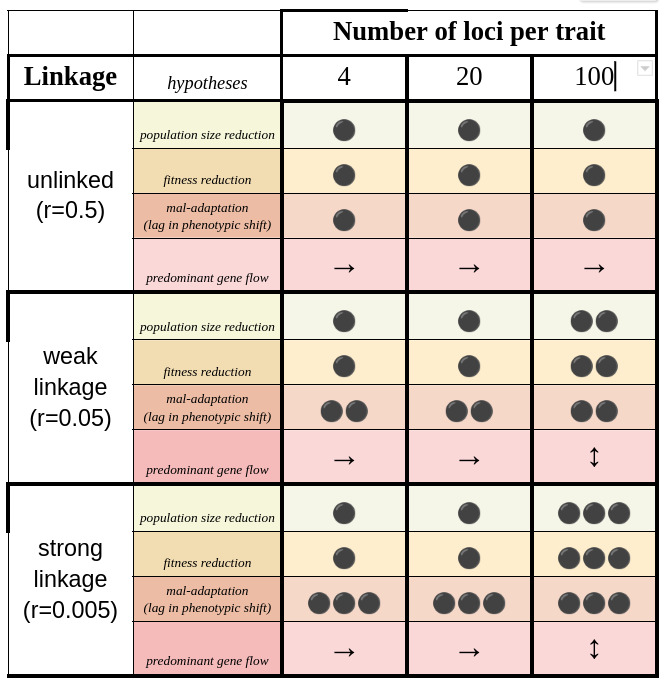
\includegraphics[width=.8\linewidth]{hypotheses}
\caption{Grid of simulation scenarios, with expected results of each based on our overall hypotheses.}
\label{tab:hypotheses}
\end{figure}



Spatially explicit simulation is one of the strongest available tools
for improving our understanding of maladaptation and adaptive capacity
under climate change \cite{capblancq_review}.
In this study, we use individual-based, spatially explicit landscape genetic simulations to
explore these key aspects of adaptation under climate change. We first simulate 
adaptation of a population to a bivariate environment composed of two horizontal 
environmental gradients, each exerting selection on a separate trait.
Individuals' trait phenotypes are determined by the additive effects of numerous loci ---
a reasonable approximation of many traits of interest in real populations \cite{sella} ---
and traits have moderate genetic redundancy 
(i.e., mid-range phenotypic values
can be generated by numerous distinct genotypes, while extreme phenotypic
values can be produced by single, extreme genotypes) and have no pleiotropy.
In our main models, we then simulate climate change on that landscape by holding one gradient 
constant while shifting the other gradient to the right, creating a situation in which
a decoupling environment drives heterogeneous natural selection toward a novel region 
of bivariate trait space. Our null models are run likewise, but without environmental 
change. We run many pairs of main and null simulations for each of nine scenarios, 
resulting from the full factorial crossing of three levels of linkage (unlinked, weak 
linkage, strong linkage) and three values for the number of genes underlying each 
trait (henceforth, ‘locus-count’; 4, 20, 100). We test a set of hypotheses, detailed 
in Table \ref{tab:hypotheses}, about the effects of linkage,
locus-count, and their interaction on key 
dynamics of the process of adaptation under climate change, including changes in 
population size and in average fitness, phenotypic shifts and the degree of 
maladaptation, and the predominant directions of gene-flow (parallel to or 
perpendicular to the direction of climatic shift). Our analysis points toward an area 
of important applied research because, to the extent that landscape genetics can cast 
light on the processes underlying maladaptation, adaptive capacity, and adaptive gene
flow, it can help answer the fundamental question posed by climate-smart management 
practices such as AGF: Whom to move where?


\section*{Results}

Population size declined during climate change across all scenarios, (GIVE ANOVA 
RESULTS) \ref{fig:Nt_over_time}, \ref{fig:Nt_boxplot}, as did mean fitness (GIVE ANOVA 
RESULTS) \ref{fig:fit_over_time}, \ref{fig:fit_boxplot}. The extent of decline was 
positively correlated with the strength of linkage, (GIVE HSD RESULTS), and 
displayed a non-linear relationship with locus count. The 100-locus scenarios showed 
extreme reductions (HSD RESULTS), with population size in the strong-linkage scenario
declining by 19\% on average (from ~10,500 to ~8000 individuals).
Notably, the population and fitness declines in the 100-locus scenarios
were also uniquely persistent, with no evolutionary rescue (i.e., no rebound occurring until climate change ceased), 
suggesting that climate change outstripped adaptive capacity in these scenarios.

Conversely, the 4- and 20-locus scenarios showed varying degrees
of decline (HSD RESULTS),
but all featured at least partial evolutionary rescue by the end of the climate change period.
Interestingly, declines were uniformly more pronounced in the 4-locus scenarios
when compared to equivalent-linkage 20-locus scenarios. DISCUSS THE 'BUMPINESS' OF THE 4-LOCUS SCENARIOS?? 
 
As expected, null simulations showed no change in population size or mean fitness. The only difference between null simulations across scenarios was a difference in the 
equilibrium mean fitness value, which is a function of locus count because locus count 
and effect size covary, and effect size dictates the proximity to which individuals can 
match the finely varying values of the continuous environmental gradients.

\begin{SCfigure*}[\sidecaptionrelwidth][t]
\centering
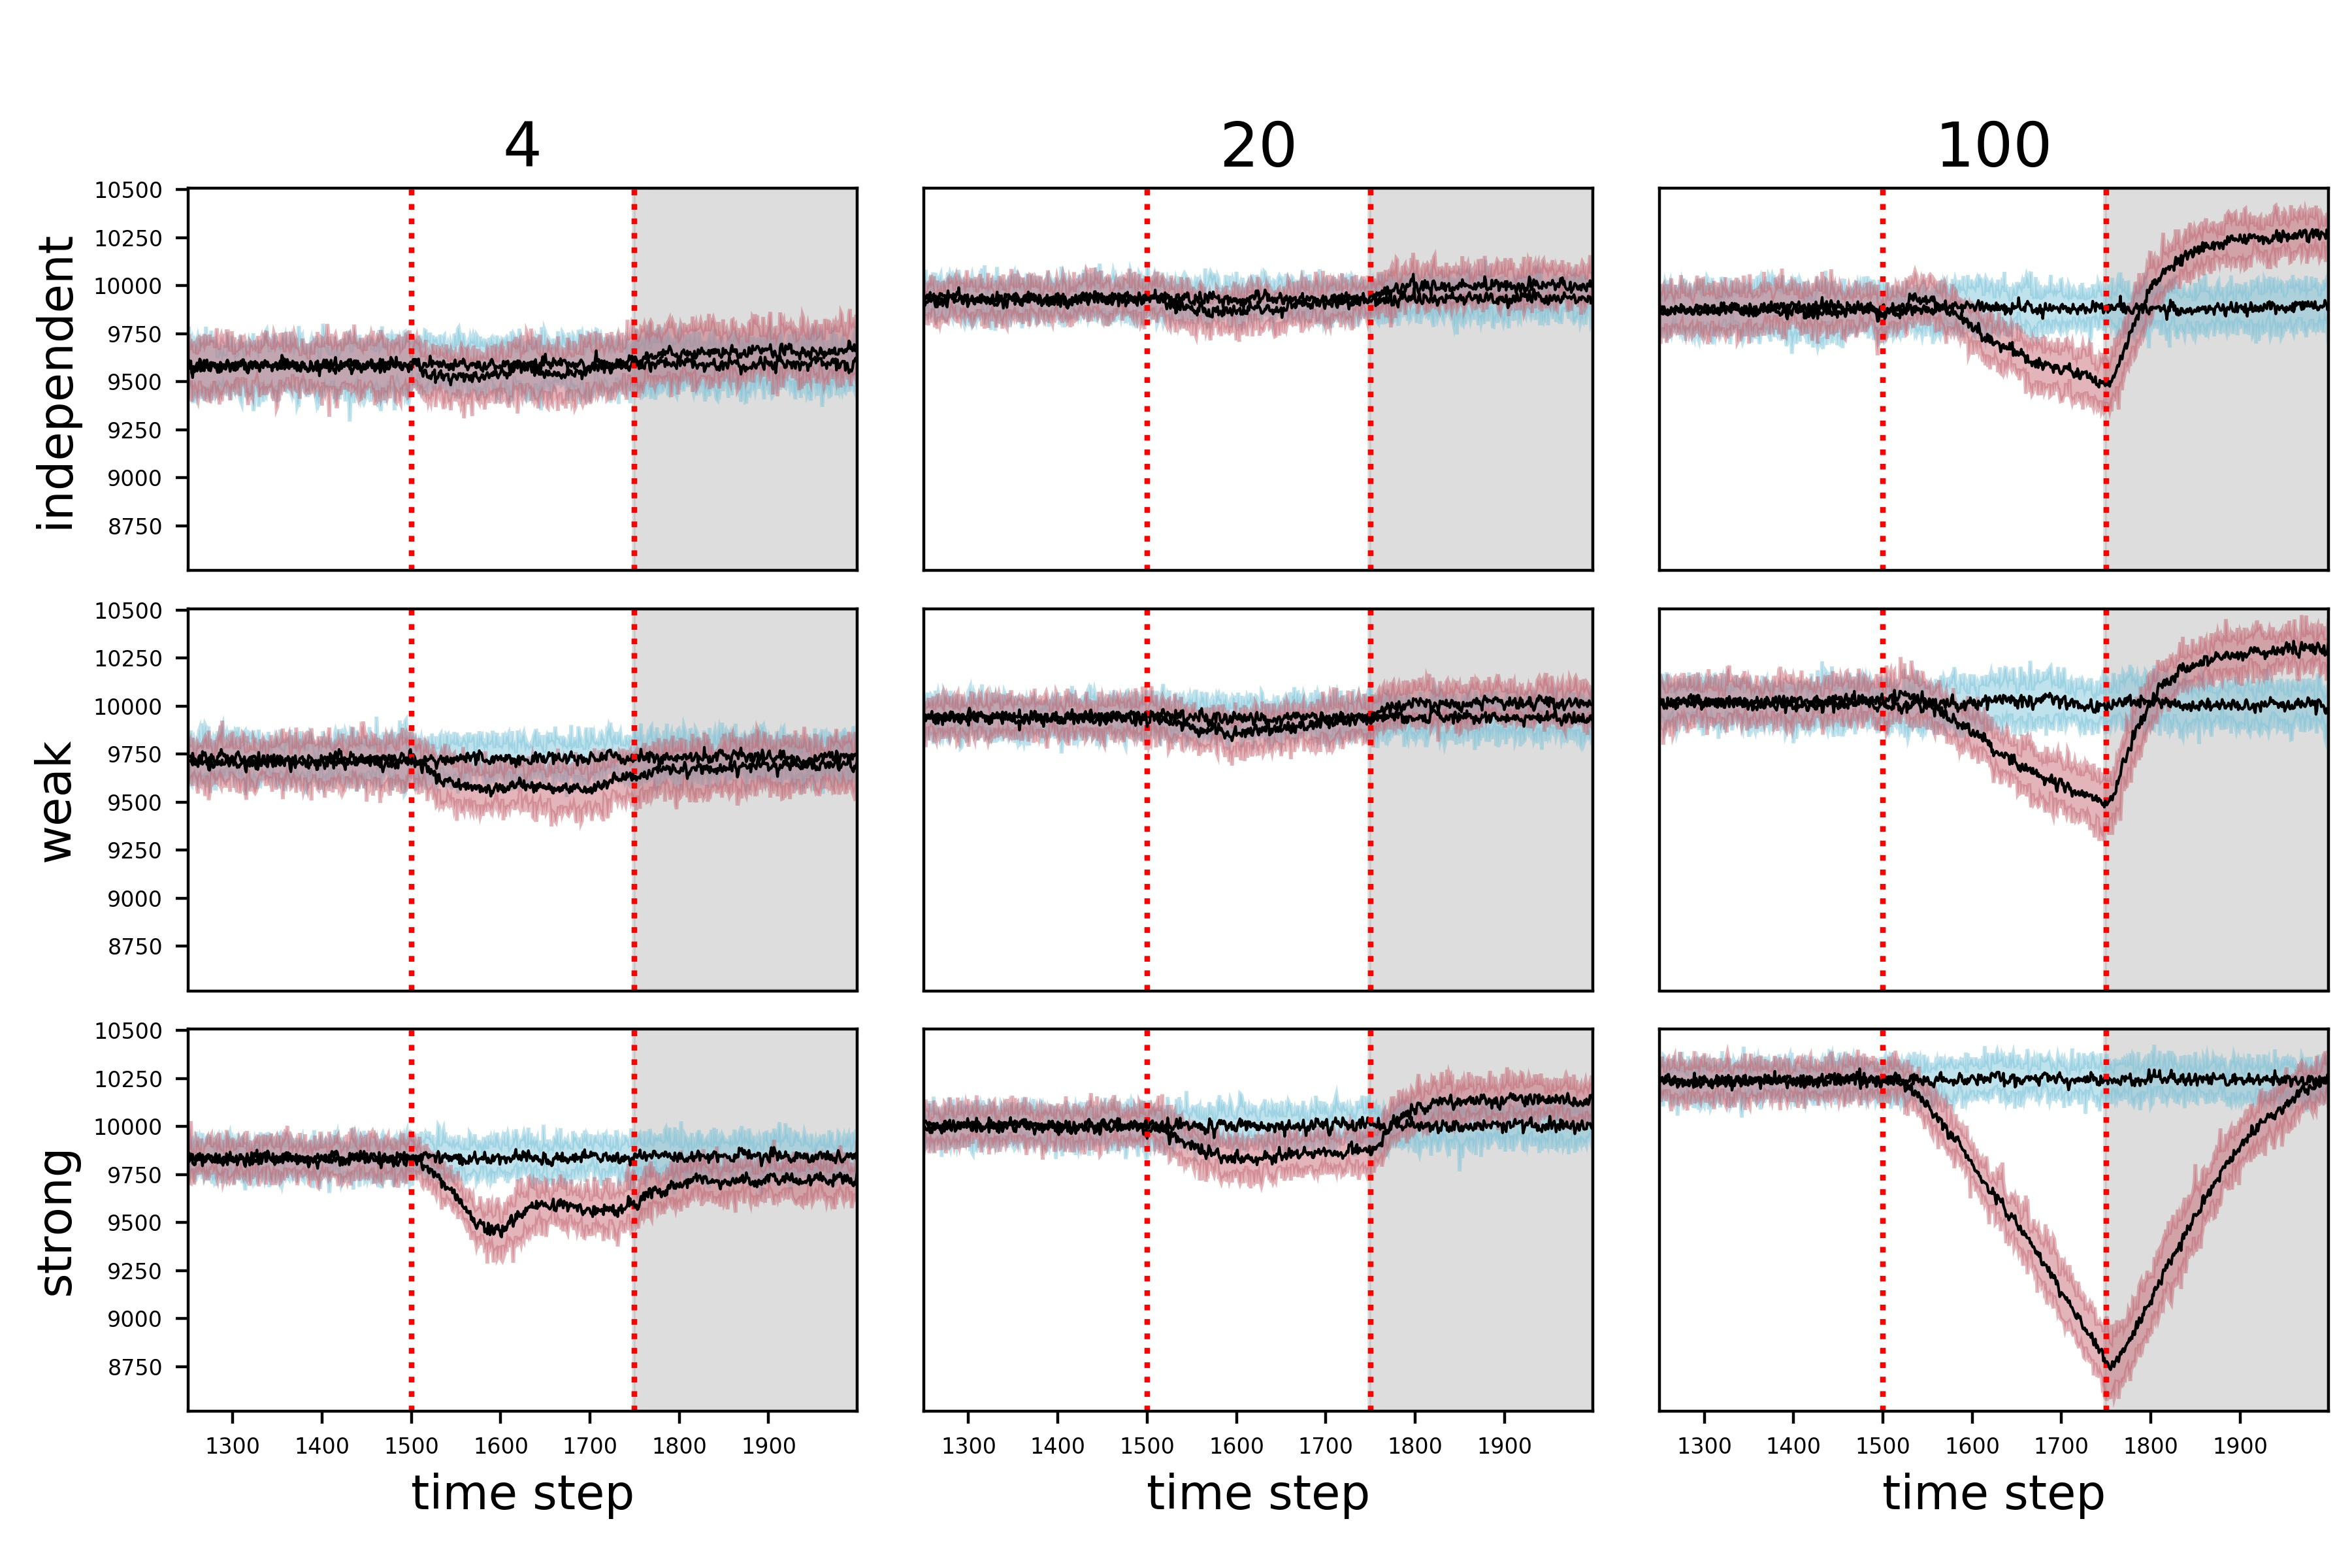
\includegraphics[width=11.4cm]{Nt_over_time.jpg}
\caption{Population size dynamics for all scenarios during the 250 time steps before the environmental change event and the 250 time steps during it (with the two periods divided by a red, dashed vertical line marking the onset of the environmental change event). Scenarios are organized as in Table 1, with rows for level of linkage and columns for number of loci per trait. Both means (black lines) and variability envelopes (5th percentile to 95th percentile) are shown, with scenario type depicted by color (main scenarios in red, null scenarios in blue).}
\label{fig:Nt_over_time}
\end{SCfigure*}

\begin{SCfigure*}[\sidecaptionrelwidth][t]
\centering
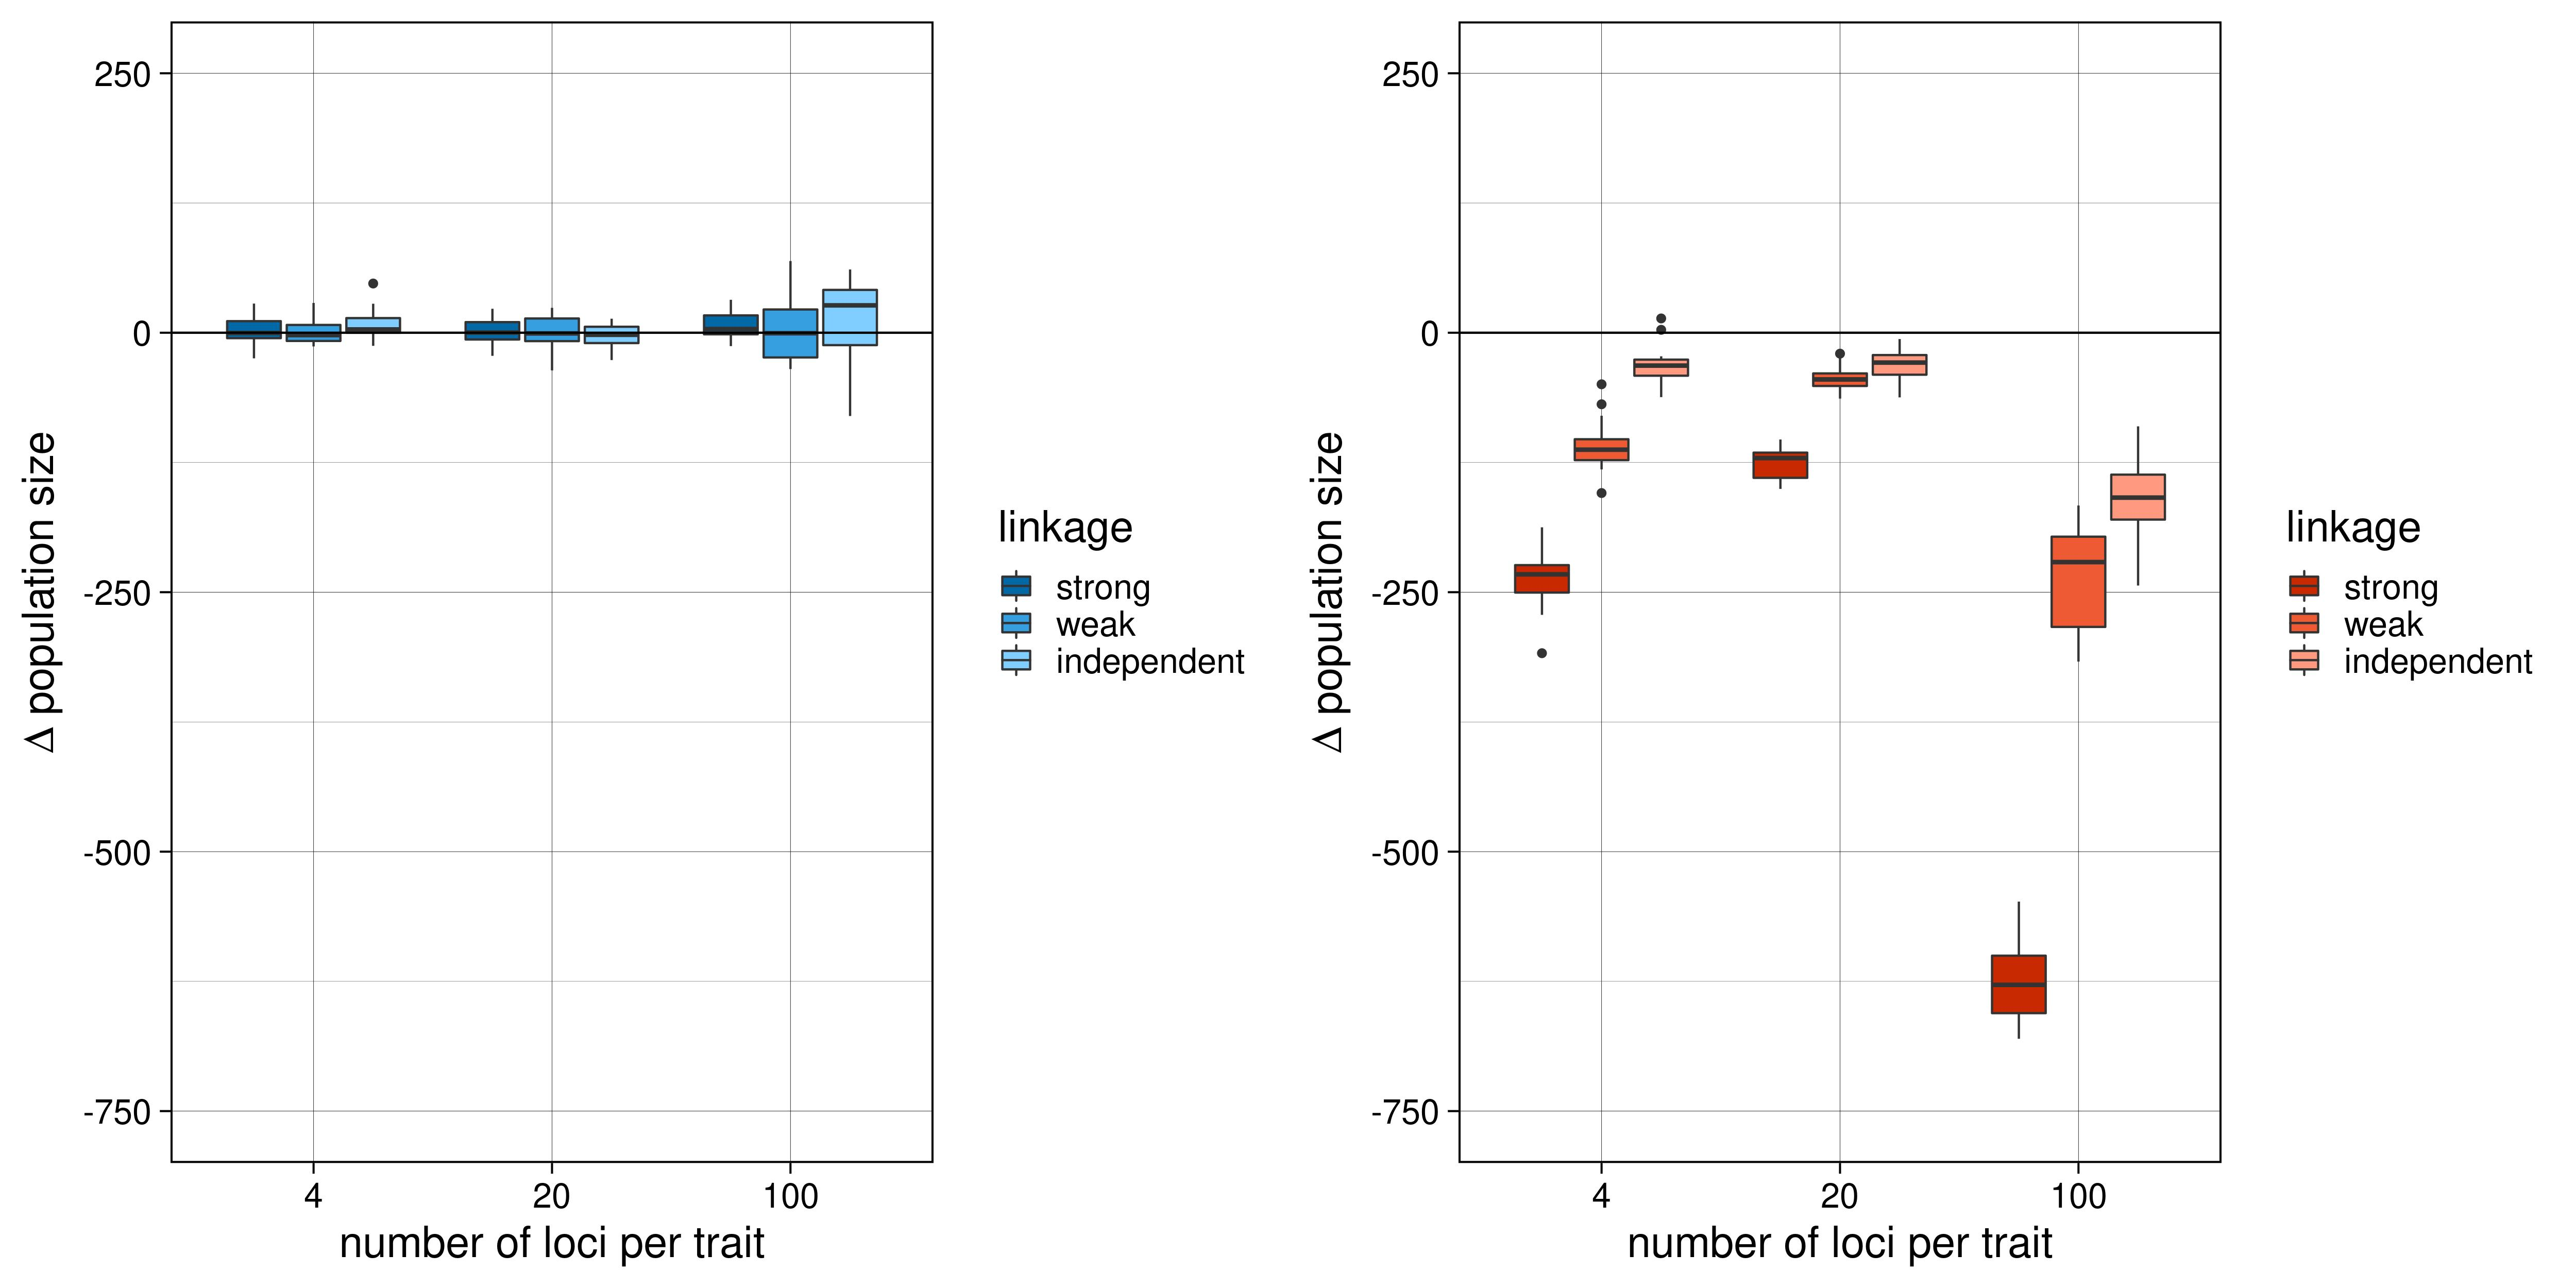
\includegraphics[width=11.4cm]{Nt_boxplot.jpg}
\caption{Boxplot comparing environmental change-driven changes in mean population size across scenarios. Null scenarios are plotted on the left in blue, and main scenarios are plotted on the right, in red. Within each plot, scenarios are divided by the number of loci per trait (x-axis) and by the strength of linkage (shade, with darker hues representing stronger linkage). Asterisks above each box indicate level of significance (*=0.1, **=0.05, ***=0.005).}
\label{fig:Nt_boxplot}
\end{SCfigure*}

\begin{SCfigure*}[\sidecaptionrelwidth][t]
\centering
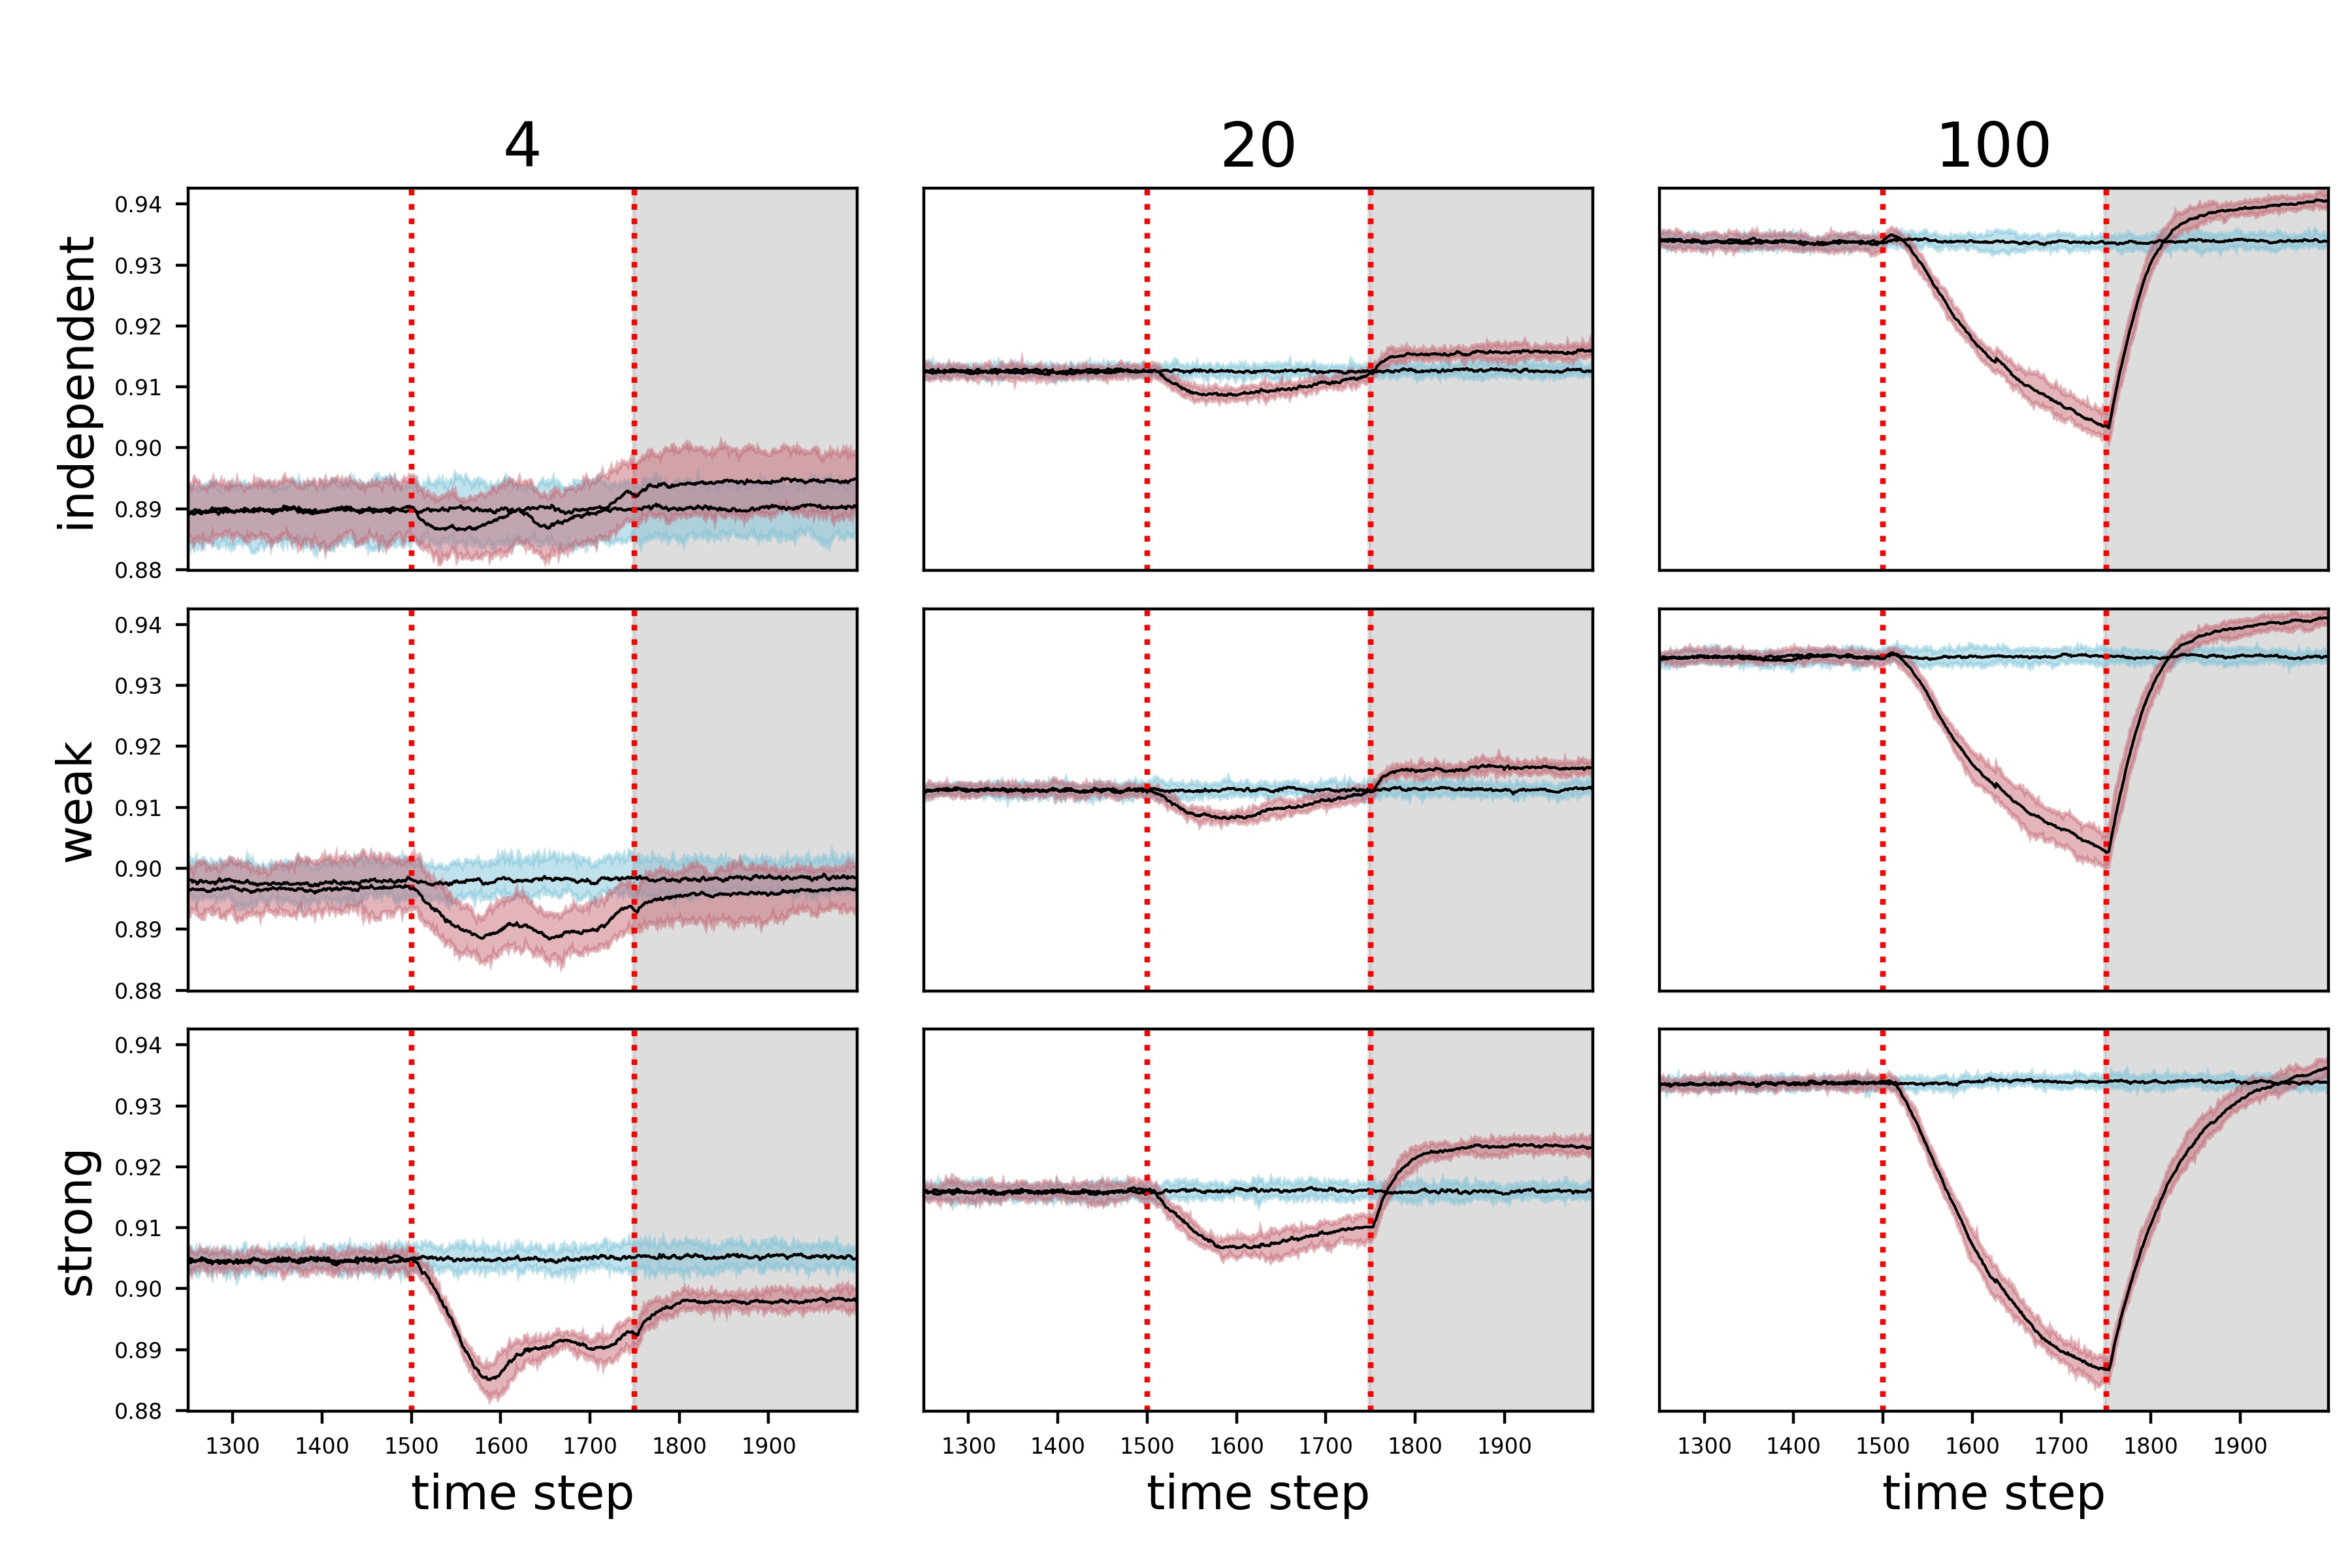
\includegraphics[width=11.4cm]{fit_over_time.jpg}
\caption{Mean fitness dynamics for all scenarios during the 250 time steps before the environmental change event and the 250 time steps during it (with the two periods divided by a red, dashed vertical line marking the onset of the environmental change event). Scenarios are organized as in Table 1, with rows for level of linkage and columns for number of loci per trait. Both means (black lines) and variability envelopes (5th percentile to 95th percentile) are shown, with scenario type depicted by color (main scenarios in red, null scenarios in blue).}
\label{fig:fit_over_time}
\end{SCfigure*}

\begin{SCfigure*}[\sidecaptionrelwidth][t]
\centering
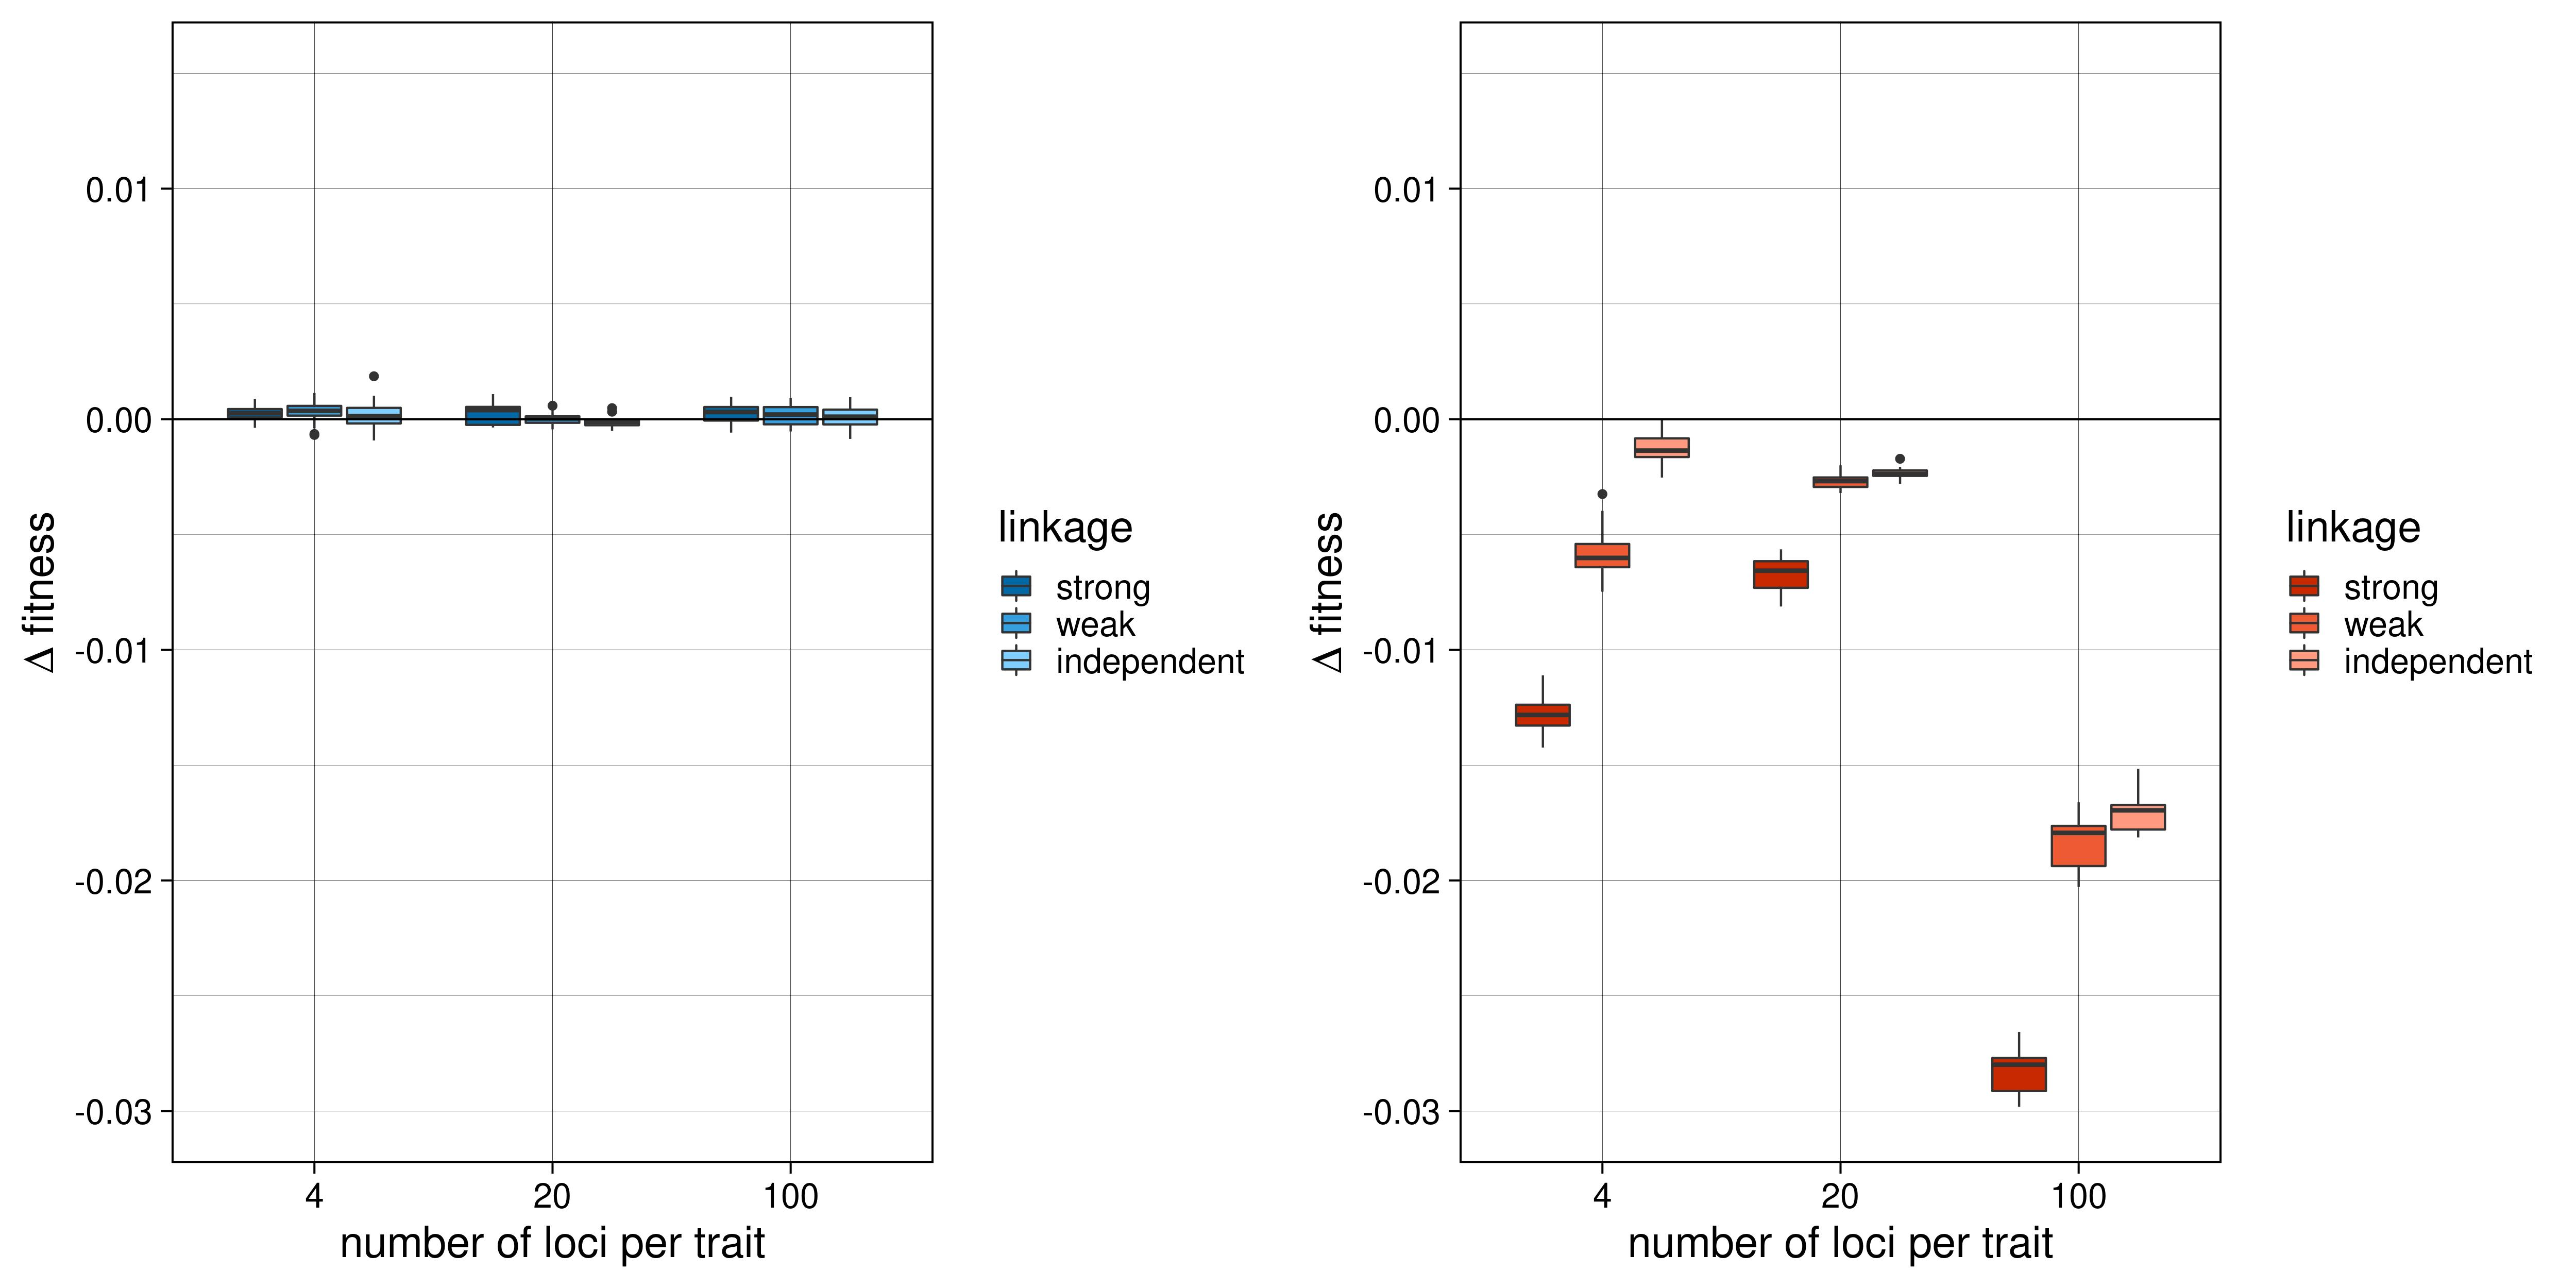
\includegraphics[width=11.4cm]{fit_boxplot.jpg}
\caption{Boxplot comparing environmental change-driven changes in mean fitness across scenarios. Null scenarios are plotted on the left in blue, and main scenarios are plotted on the right, in red. Within each plot, scenarios are divided by the number of loci per trait (x-axis) and by the strength of linkage (shade, with darker hues representing stronger linkage). Asterisks above each box indicate level of significance (*=0.1, **=0.05, ***=0.005).}
\label{fig:fit_boxplot}
\end{SCfigure*}

All scenarios displayed some maladaptation, as evidenced by the red 'phenotypic shortfall' wedges shown in the 'after' scatterplots in Figure \ref{fig:pheno_shift}. However, maladaptation was significantly higher in the 100-locus scenarios, and especially when linkage was strong.
In these scenarios, maladaptation was so strong that local extinction occurred
in the fastest-changing, eastern extreme of the landscape,
as evidenced both by the emptiness of the bottom-central portions
of the rightmost scatterplots in Figure \ref{fig:pheno_shift}
(as well as the before-after comparisons of population density plotted in
Figure SX).


\begin{figure*}
\centering
\includegraphics[width=17.8cm]{pheno_shift.jpg}
\caption{Comparison, across all nine scenarios, of the observed versus expected phenotypic shift during the environmental change event. Scenarios are organized as in Table 1, with rows for level of linkage and columns for number of loci per trait. For each scenario, the left scatterplot shows the distribution of individuals’ bivariate phenotypes before the environmental change event begins (‘before’ columns), whereas the right scatterplot shows how the distribution has shifted by the end of the environmental change event (‘after’ columns). The trait adapted to the shifting environmental gradient is distributed along the x axis, and the trait adapted to the stable gradient is distributed along the y axis. Scatterplots depict multi-model ensemble results for each scenario. The size and opacity of each point represents the number of individuals exhibiting that bivariate phenotype. (Note that the gridded arrangement of the points in each scatterplot is a function of the number of loci per trait which, because locus effect sizes are fixed, directly determines the set of attainable, evenly-spaced, discrete phenotypic values. Because fewer loci per trait yields fewer possible phenotypes, individuals are grouped into fewer, larger phenotypic bins in the 4- and 20-locus scenarios.) Solid black lines delineate the shift in the phenotypic distributions’ central tendencies that is expected to take place during the environmental change event, dotted black lines depict the observed (OLS-fitted) phenotypic distributions’ central tendencies at the ‘during’ and ‘after’ time steps, and translucent red wedges depict the differences between the expected and observed distributions (i.e., ‘phenotypic shortfall’, the response variable in our statistical tests).
}
\label{fig:pheno_shift}
\end{figure*}

In our null simulations, gene flow distributions varied across scenarios in a systematic way. On-contour (i.e., north/south) gene flow increased relative to up-gradient (i.e., east/west) gene flow as a function of strength of linkage, and did so most strongly in the 4-locus scenarios (GIVE ANOVA AND HSD RESULTS). Against this background expectation, up-gradient (i.e., eastward) gene flow was greater in main than null simulations for all scenarios.  The scenarios with the strongest on-contour gene flow (strong-linkage 20-locus, and weak- and strong-linkage 4 locus) still retained a signature of great-than-uniform on-contour gene flow despite adaptation to climate change. As expected, down-gradient (i.e., westward) gene flow was depressed relative to the null in all main scenarios.


\begin{figure*}
\centering
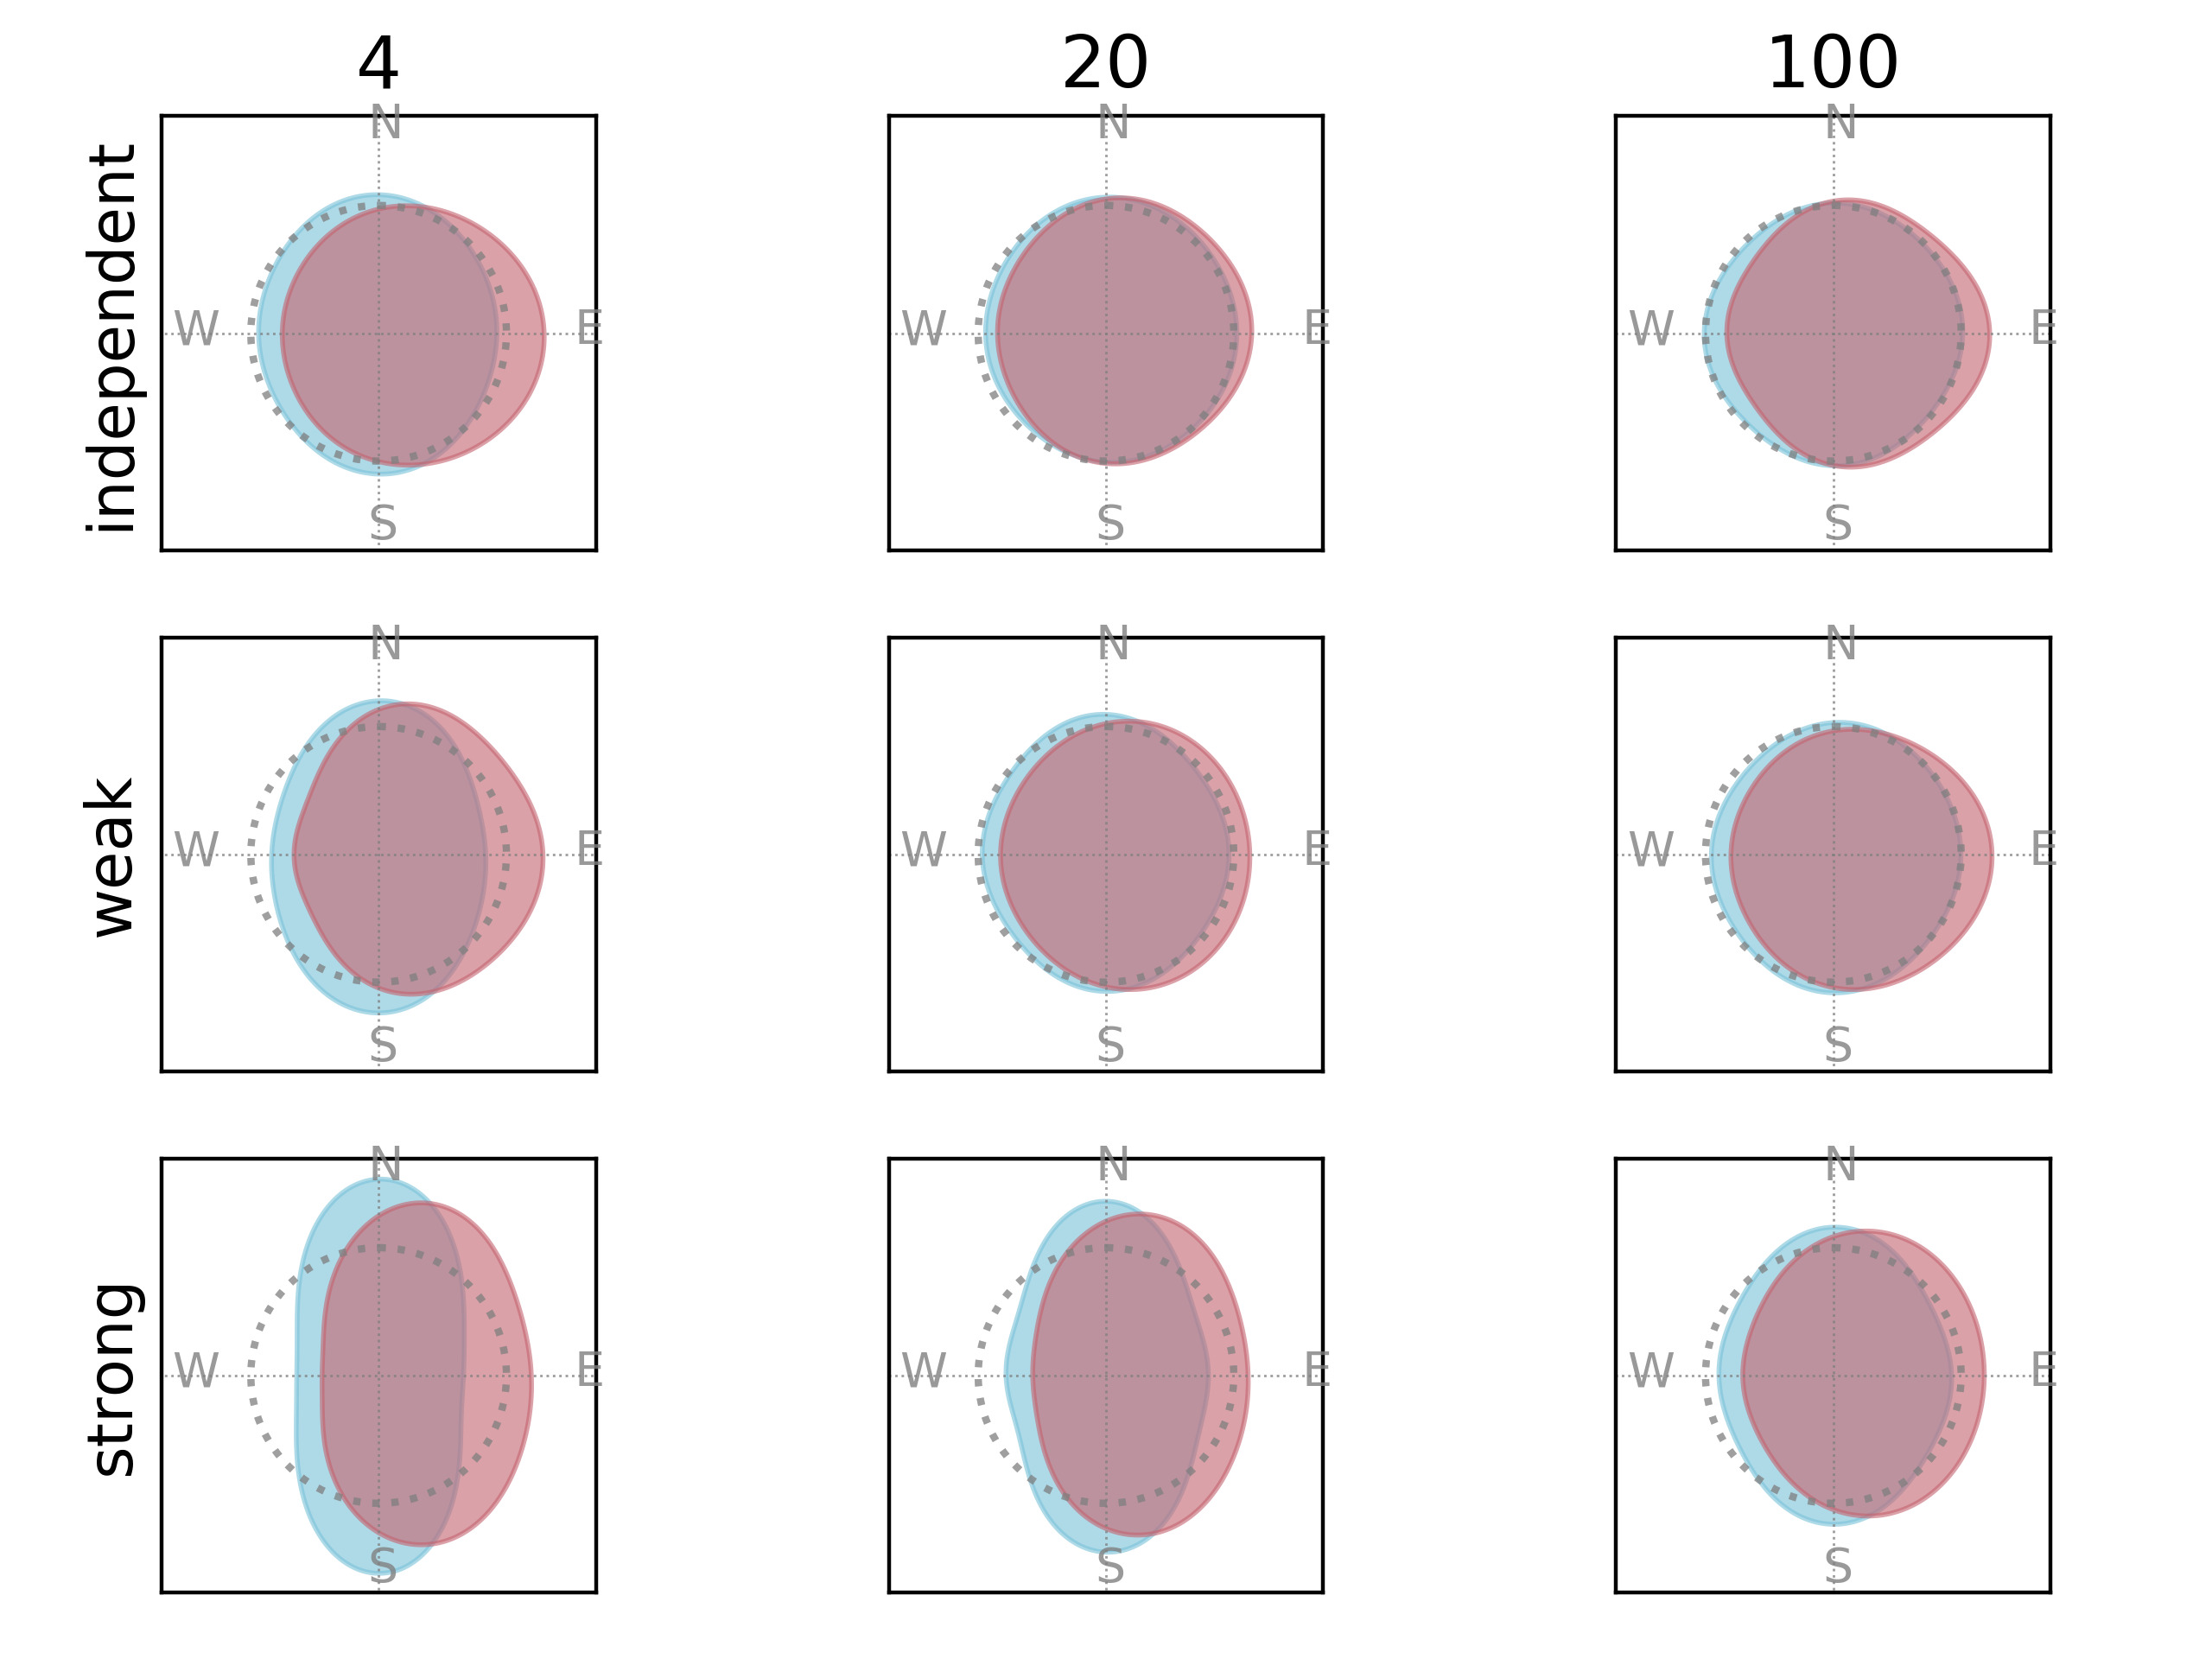
\includegraphics[width=17.8cm]{gene_flow.jpg}
\caption{Comparison, across all nine scenarios, of the distributions of gene-flow directions during the environmental change event. Scenarios are organized as in Table 1, with rows for level of linkage and columns for number of loci per trait. Main scenarios (red) are compared against null scenarios (blue). Compass labels indicate directions of gene flow as it would be observed from a bird’s-eye view of the simulated landscape, with eastward gene flow moving in the same direction as the shifting environmental gradient (i.e., ‘upslope’), and with northward and southward gene flow being perpendicular to the environmental gradients (i.e., ‘on contour’). Westward gene flow would go against the direction of the shifting environmental gradient, and thus would be maladaptive under all scenarios, which explains why it is universally suppressed relative to the null results. There is a general trend toward increasing on-contour gene flow and decreasing upslope gene flow with increasing strength of linkage and increasing number of loci per trait..
}
\label{fig:gene_flow}
\end{figure*}


\section*{Discussion}
The generalized pattern of population and fitness decline under climate change match the
overall trend expected under our hypotheses and under first-order theory of
the evolutionary impact of climate change \cite{aitken_whitlock}.

The trends of these declines across also generally matched our hypotheses,
with the degree of decline being positively correlated with linkage and with locus-count.

Similarly, the trends in phenotypic shift and maladaptation
across the scenarios generally matched our hypotheses,
but the degree of maladaptation was much more sensitive to
locus-count than to linkage.
The time courses in Figures \ref{fig:Nt_over_time} and \ref{fig:fit_over_time} help explain this: declines
are stronger with stronger linkage, but evolutionary
rescue is still successful, such that our metric of maladaptation,
measured at the end of the climate change period,
fails to reflect this dynamic.
To the contrary, the 100-locus scenarios,
in which adaptive capacity is outstripped,
show substantial maladaptation at the end of the climate
change period, to such an extent that the fastest-changing
eastern section experiences local extinction.

However, the dramatic degree of population decline observed in the 100-locus scenarios was unexpected,
especially given that adaptive capacity was outstripped in all scenarios, irrespective of 
linkage.

We expected evolutionary responses to be slower for higher locus-count architectures
because of the smaller effect size of individual loci and, in the linked scenarios,
the long expected wait times
until recombination produced adaptive clusters with larger effective effect sizes.
But we did not expect a complete failure to adapt.

Our work makes significant contributions to the theoretical understanding of 
adaptation to complex and changing environments.
Theory indicates that recombination can be deleterious
in situations of adaptation with gene flow
along a gradient, because it disrupts the association between adaptive loci 
underlying a single trait \cite{tigano}.
Our results highlight an interesting interesting and important context for that expectation:
It applies in the special case of a single-trait adapted to a single gradient,
but may change under other realizations of the
a generalized $n$-trait, $m$-gradient model.
In our two-trait, two-gradient model, given that the gradients decouple
and novel environmental space emerges,
recombination proves to be net-advantageous.
This is because, although recombination does disrupt the association between
adaptive loci for the shifting gradient's trait, preventing the
generation of larger-effect gene clusters,
it simultaneously dissociates those loci from the loci underlying
the stable gradient's trait, for which gene flow would be maladaptive.
In other words, recombination facilitates adaptation by gene flow
by precluding interference between two complex genetic architectures.
   
Our work also has important management implications.   

Given that our 20-locus scenarios showed little to no decline in population size and mean fitness, our results seem to contradict previous findings that adaptation on a cline tends to occur either by few genes of large effect or by many genes of small effect \cite{yeaman_amnat}. This apparent contradiction may be partly explained by a difference in timeframes between adaptation to a static environmental gradient and adaptation to an ongoing shift in a multivariate gradient. Adaptation to a single, static gradient can proceed gradually, and may favor large-effect alleles or, large-effect clusters of small-effect alleles, once they arise by mutation, recombination, gene flow, or some combination. To the contrary, the sudden onset of persistent environmental perturbation in a population that is already locally adapted initiates a 'race against time', and it may be the case that 'middle of the road' genetic architectures --- those composed of freely recombining loci with small-enough effect sizes to escape large sudden declines in fitness, but with large enough effect sizes to avoid the long wait times necessary for recombination to cluster many adaptive loci into larger-effect haplotypes  -- will fair best. In theoretical models, local adaptation with migration along static gradients tends to favor concentrated genetic architectures featuring linked clusters of large-effect alleles. To the contrary, there is some indication that temporally fluctuating environments favor dispersed genetic architectures with higher rates of recombination \cite{burger,kondrashov,yeaman_review,yeaman_whitlock}. This suggests an inherent tension between the architectures that might arise in natural populations and the architectures likely to facilitate adaptation of those populations to rapid environmental change --- though it remains to be determined how often and when concentrated genetic architectures actually occur in real-world systems \cite{laruson}.  This suggests a mechanism by which species living in climates with less interannual fluctuation and longer-term stationarity could have higher intrinsic vulnerability to maladaptation under climate change, all else equal.
   

   \begin{enumerate}
        \item in all scenarios, up-gradient gene flow increases because of climate change --> suggests that even if maladaptive, less so than only \textit{in situ} evolution --> supports the concept of AGF
        \item Adaptive capacity was outstripped in the 100-locus scenarios, even when recombination was free. These are likely to be the most realistic scenarios, given the polygenic nature of many complex ecological traits \cite{barghi_polygenic}. What does this suggest for conservation concerns? what future research would be necessary to inform them? how realistic these parameterizations are? and to the extent they are, given the difficulty and expense of obtaining functional genetic information in most wild study systems, what are possible indicators of study systems under such circumstances? --> those systems would be major candidates for AGF --> could be trees and other long-lived, foundational species, as previously suggested \cite{aitken_whitlock, aitken_bemmels}
        \item many ecological traits of interest are polygenic, and it is a reasonable default assumption that all environments are multivariate, with traits adapted to multiple aspects of the environment that are differentially distributed in space and that change differentially over time
        \item While it is exceedingly hard to document and understand the nature of adaptation to a multivariate environment in a wild study system, and thus to make management decisions on such a basis, it is nonetheless important to keep in mind the caveat that not all adaptation climate change is bound to look like upslope gene flow, and conversely, that not all upslope gene flow is bound to facilitate adaptation to climate change.
    \end{enumerate}

The major challenge in simulation-based research is the complexity of the high-dimensional 
parameter space that can be explored. Informative studies can be constructed by focusing on a 
small set of key parameters and exploring their influence
on the outcomes of interest, while holding other parameters at reasonable values. We have 
attempted to do that here. Nonetheless, some of the parameters we held constant here are certain 
to have important effects, the elucidation of which would provide a more comprehensive 
mechanistic picture of the nature of adaptation to environmental change. The foremost of these, 
which are areas ripe for future research, are:
    \begin{enumerate}
        \item \textit{population size}, a key determinant of the relative strengths of drift and natural selection \cite{murray} and of the wait time to emergence of recombinant haploytpes \cite{christiansen}, among other important dynamics;
        \item \textit{migration} (as either a fixed distance or a distribution \cite{paulose}), a key factor embedded in the rudimentary migration-selection dynamics that lie at the heart of models like ours \cite{wright,haldane,barton}, and the fundamental process motivating the practice of AGF;
        \item \textit{genetic redundancy} \cite{barghi_redundancy,barghi_polygenic,laruson} , both of which could be varied in order to investigate the evolution of complex genetic architectures and convergent adaptation, and their effects on adaptive capacity to environmental change.
    \end{enumerate}
    A variety of other facets of spatiotemporal evolution could also be explored through a similar modeling framework, including fixed versus distributed allelic effect sizes \cite{orr} and genomic positions; plasticity \cite{chevin} and heritable epigenetic variation; pleiotropy \cite{thompson}; more complex spatial arrangements \cite{benes}; and mutation (although the relevance of \textit{de novo} mutation to climate change adaptation in many of the relatively long-lived and long-generation-time species of conservation concern is an open question).
    Finally, important, conservation-relevant insight could emerge from the integration of other dimensions climate change ecology, including range shifts \cite{weiss-lehman}, variable distributions of population density \cite{aitken_whitlock}, and comparisons between variably steep climatic gradients, variable rates of climatic change, and between scenarios in which rates of climate change are spatially stationary or variable. 





\matmethods{

\subsection*{Simulation}

We built all of the simulations for this study using \texttt{geonomics} \cite{terasaki_hart},
a Python \cite{rossum} package for
creating forward-time, agent-based, continuous-space landscape genomic simulations 
using arbitrarily complex life histories, environments, and environmental change 
scenarios. We created a base scenario for our set of simulations
by creating a \texttt{geonomics} template
parameters file featuring a species with two traits, each of which experiences 
selection on the basis of a different environmental variable (using the \texttt{geonomics.make\_parameters\_file} command).
Both environmental variables are modeled as linear, horizontal gradients
that span environmental values from 1 to 0, west to east.
During the simulation, one of these layers undergoes an environmental change 
event in which the gradient’s values change stepwise, over 250 time steps,
resulting in a final gradient that spans values from 1 to 0.5, west to east.
This creates a scenario in 
which two environmental variables become decoupled, leading 
to the emergence of novel environments (i.e. sites occupying new vectors in 
two-dimensional environmental space). Our goal here was to emulate a common 
phenomenon under climate change: the emergence of novel climates \cite{williams_novel_climates,williams_projected_novel_disappearing,fitzpatrick_climate_novelty_forecasts}.

Importantly, this landscape arrangement also generate heterogeneous rates of climate change,
with the rate ranging from 0 at the western edge to $0.5/250 time steps$ at the eastern edge.
This complicates interpretation of our results,
but much less so than in an alternative scenario
with spatially homogeneous rates of change,
which would have experienced range expansion as well as adaptation
during the climate change period.
The latter approach is also of interest,
and will be explored in future work,
but the approach we chose here allowed us
to best isolate evolutionary dynamics
resulting from the components of genetic architecture
that define our scenarios and hypotheses.

We then wrote a custom script in Python that reads that template \texttt{geonomics}
parameters file, 2.) edits any parameters that vary 
across our scenarios, 3.) instantiates a model, 4.) runs a fixed number of iterations 
of that model, and 5.) outputs custom data of interest. The parameters of interest, 
and the values they were assigned, were: the number of loci underlying each trait 
(parameter \texttt{n\_loci}: low = 5, moderate = 20, high = 100), and the linkage between 
neighboring loci (i.e., the homogeneous recombination rate parameter, parameter \texttt{r}: unlinked = 
0.5, weak linkage = 0.05, strong linkage = 0.005).
(We did not include neutral loci in the simulations because genetic
hitchhiking would prevent them from providing unique information
in all but the unliked scenarios.)
The full factorial combinations
of the chosen values of those parameters generate the set
of simulation scenarios laid out in
the central grid of Table 1. We used that script to run a set of batch jobs on the 
savio3 partition of UC Berkeley’s Savio system (each node has 96 GB RAM and 32, 
2.1-GHz Skylake processors). For each scenario, we ran a total of 250 iterations of 
the scenario of interest, featuring a 250-time-step environmental change (henceforth, 
the ‘main’ scenarios), and 250 iterations of a paired null scenario without natural 
selection (henceforth, the ‘null’ scenarios). 


Given that \texttt{geonomics} is a complex simulation framework, it features numerous other 
parameters whose values could be set or explored by the user. For the vast majority of
these parameters we left them set at reasonable default values. However, the 
parameters that we deemed as having high potential influence over results despite not 
being of particular interest for our study (henceforth, ‘nuisance parameters’) were 
set to low, high, and middle values within a reasonable range. NUISANCE PARAMETERS 
INCLUDED… This generated independent datasets for each value of each nuisance 
parameter. We reran our main analyses, as explained below, for each of these 
independent datasets, allowing us to characterize sensitivity of our results to each 
nuisance parameter. (For the complete set of \texttt{geonomics} parameters, and the values 
assigned to them across all models, see Appendix XXX.) ORGANIZE THIS APPENDIX AS A GNX
PARAMETERS FILE WITH MULTIPLE VALUES DISPLAYED AND HIGHLIGHTED IN GREEN FOR KEY PARAMS
OF INTEREST AND MULTIPLE VALUES DISPLAYED AND HIGHLIGHTED IN ORANGE FOR NUISANCE PARAMS.


Using a combination of internal \texttt{geonomics} functions and custom Python code, we 
designed a set of data outputs from each model run that would allow us to test our 
series of hypotheses. We saved tables of individuals’ locations and phenotypes at both
the beginning and the end of the environmental change period. We also saved time 
series of population size, mean fitness, and mean phenotype of the trait adapted to 
the shifting gradient. We gathered this data at every time step, from 250 time steps 
before the environmental change event, through the 250 time steps of the event, and 
continuing until 250 time steps after the event completed. 
Lastly, we saved data on the vector directions of all gene flow during the 
environmental change event, extracted from the spatial pedigrees stored in the
\texttt{tskit} \cite{kelleher} 
data structures. From that full set of gene flow data we calculated a pair of measures
of gene flow directionality,  which we refer to as ‘eastness’ (i.e., up-gradient 
directionality) and ‘north-southness’ (i.e., on-contour directionality). These were 
calculated as:

$Eness = \frac{\sum\limits_{i}^{n}\cos\theta}{n},\ \cos\theta\geq0$,

$NSness = \frac{\sum\limits_{i}^{n}|\sin\theta|}{n}$,

where angles are expressed counterclockwise from east. We ignored westness because 
gene flow in that direction is expected to be low irrespective 
of scenario, given that it would oppose the environmental shift and would almost 
always be maladaptive. We also saved a subsample of the full set of gene flow 
direction data by keeping all data pertaining to two randomly chosen loci that had 
positive effects on the trait adapted to the shifting environmental gradient. We 
restricted our sample in this way both to focus on loci expected to facilitate 
adaptation to increasing environmental values and thus to shift upslope, and to 
provide equal sample sizes across scenarios in downstream analysis (which was 
constrained to the number of positive-effect loci present in the four-locus-per-trait 
scenarios, i.e. two). 


For each of our nine scenarios, and for both main and null scenarios, we ran 250 
iterations and generated 250 of the output data sets described above. We then 
generated visual summaries and ran statistical analyses across all simulations’ 
datasets. All analysis and visualization was produced using custom scripts written in 
Python and R \cite{r_core_team}.

\subsection*{Analysis}

DESCRIBE ALL ANALYSES OF RESULTING DATA

To probe our hypotheses about environmental change-driven shifts in population size, 
mean fitness, and mean phenotype of the shifting-gradient trait, we first plotted the 
trajectories of these metrics in each of our nine scenarios. For each scenario, and 
for both main and null models, we created ensemble datasets by combining all 250 
iterations’ population size and mean fitness time series outputs. For each time step 
in the time series we calculated the mean and the 5th and 95th percentiles. Then we 
plotted, across all scenarios, the resulting trajectories of the means and their 
variability envelopes, for population size (Figure 1), mean fitness (Figure 2), and 
mean phenotype of the shifting-gradient trait (Figure S1). We plotted these metrics 
from 250 time steps before the environmental change event until 250 time steps after 
its completion, allowing us to visualize the onset, course, and aftermath of the 
change event. 


To test our hypotheses about population size and mean fitness, we calculated a single 
metric of change over the course of the environmental change event (, where x can be 
either population size or mean fitness) for each run of each scenario. We then ran a 
two-way ANOVA of each one, partitioning variance as a function of the two independent 
variables that defined our scenarios (number of loci per trait; strength of linkage). 
We ran post hoc Tukey’s honest significant difference (HSD) tests each time an ANOVA 
showed overall significant results, to determine which levels of our independent 
variables showed divergent results. Lastly, we repeated this analysis for all null 
simulations, as a control.


To test our hypotheses about the pace of phenotypic shift across scenarios, we 
developed a metric of ‘phenotypic shortfall’, then compared it across our grid of 
scenarios. We defined ‘phenotypic shortfall’ as the difference between: a.) the area 
within two-dimensional trait space that the population’s phenotypic distribution 
should have shifted across during the environmental change event so as to remain 
optimally fit to its environment, and b.) the observed area of phenotypic shift within
a simulation. To measure this area, we first determined the triangular area between 
the expected central tendency line of the optimal bivariate phenotypic distribution 
before the environmental change event and the same line of optimal distribution after 
the event. The expected central tendency lines that delineate this area are clearly 
set by the model parameterization: they are the lines connecting all of the discrete 
points in environmental space that occur on the pre- and post-change landscapes. For 
each model run, we used ordinary least squares (OLS) to fit a best-fit trend line to 
the observed phenotypic distribution of the population at the end of the environmental
change event (arithmetically fixing the y-intercept at the (1,1) point in phenotypic 
space, which is the unchanging phenotypic optimum at the righthand extent of the 
landscape). We then calculated the phenotypic shortfall as the area of the wedge 
between the expected and observed post-change central tendency lines of the 
population’s phenotypic distribution. We calculated phenotypic shortfall for each 
model run, then used two-way ANOVA to test for a difference of means as a function of 
number of loci per trait and strength of linkage. Additionally, we used post-hoc HSD 
tests to further explore the observed differences in phenotypic shift across our 
scenarios. Finally, we used the ensemble data from all model runs to visualize this 
analysis in Figure XXX, including the observed phenotypic distributions before, 
during, and after environmental change (scatterplots), expected distributional central
tendencies before and after change (solid lines), observed central tendencies (dotted 
lines), and observed phenotypic shortfalls (translucent red wedges).
	

To visually investigate our hypothesis about the predominant directionality of gene 
flow under each scenario, we first produced a visualization of the directional 
distributions of gene flow in all 9 scenarios, compared between main and null 
scenarios (Figure 7). From each model run we gathered directional data for a random 
sample of the gene flow that occurred during the environmental change event, using 
\texttt{geonomics} integration with \texttt{tskit} \cite{kelleher}, which allows for temporal 
subsetting and output of the information contained the full spatial pedigree of a 
population. We then fitted a mixture of 4 von Mises distributions to that data, 
yielding 12 parameter estimates defining the fitted mixture distribution. For each of 
the nine scenarios, we then plotted the mean of the probability density functions 
described by each of those length-12 vectors of fitted parameters. We did this 
separately for null scenarios and for main scenarios, then overlaid the null and main 
results, providing a summary depiction of the nature of gene flow within each 
scenario, compared to its null expectation.


To test our hypotheses about the direction of gene flow, we ran two-way ANOVAs of 
eastness and north-southness (with Bonferroni correction for multiple testing), 
followed by post hoc HSD tests. We also ran this analysis for null simulations, as a 
control.

} % end matmethods

\showmatmethods{} % Display the Materials and Methods section

\acknow{We thank T. Dawson,  J. Frederick, N. Graham, M. Kelly, M. McElroy, E. Westeen, G. Wogan, and M. Yuan for feedback and guidance on various iterations of the simulations presented herein. We thank Berkeley Research Computing for providing access to the Savio computing cluster. We thank D. Ehrenfeld, N. Fefferman, M. Fitzpatrick, and L. Plough for cultivating an interest in conservation genetics. Lastly, we thank M. Terasaki Hart, C. Nemec-Hart, G. Hart, J. Hart, and M. Tylka for supporting and encouraging a lifetime of curiosity about nature, and C. S. aTunde Adjuah, B. Evans, R. Pérez Joglar, Y. Y. Ma, and J. Redman for the pleasant solitude. This work was supported by a Berkeley Fellowship (to D.E.T.H.) and National Science Foundation grant DEB1845682 (to I.J.W.).}

\showacknow{} % Display the acknowledgments section

% Bibliography
\bibliography{terasaki_hart_ch2}

\end{document}